\chapter{Versuchsdurchführung und Aufbau}
Damit die FRET-Effizienz Messungen möglich und beobachtbar sind, benötigt man ein konfokales Laser-Scanning-Mikroskop.
In unserem Fall ist das Konfokalmikroskop vom Typ Leica TCS SP5, welches durch ein Computer-Messprogramm steuerbar ist. Am Mikroskop ist das Objektiv 
HCX PL APO lambda blue 63.0 x 1.4 OIL UV befestigt. 
Die zwei Laserlinien des Argon-Ionen-Laser 
dienen zur Anregung und haben die Wellenlängen 458 nm und 514 nm. Die Laserintensitäten 
wurden auf 30\% bei 458 nm und auf 3\% bei 514 nm eingestellt.
Die Detektion geschieht durch zwei Photomultiplier (PMT). Das erste PMT detektiert 
eine Wellenlängenbreite von $470\,$nm bis $500\,$nm, das zweite PMT einen Bereich von $520\,$nm bis $550\,$nm.
Zur besseren Veranschaulichung ist die Abbildung \ref{fig:laserlinien} eingefügt.\\
Das oben erwähnte Messprogramm musste vor dem Versuch eingestellt werden, hierzu 
wurden einige Probemessungen durchgeführt, um die richtigen Parameter für den Verlauf des Versuches
festzulegen. 
Dabei wurde eine Pinhole-Größe von 2,0 AU bestimmt, damit die Auflösung und die Intensität das
richtige Verhältnis haben.
Der Smart-Gain wurde konstant 
auf 1000.0 V gestellt und der Offset auf 0\%. 
Als nächstes wurde die Bildgröße bestimmt, eine höhere Bildgröße
führt zu einer besseren Auflösung, allerdings ist diese auch mit einer 
längeren Messdauer verbunden.  Somit wurde die Bildgröße von \newline 512 x 512 Pixel als ausreichend für unseren
Versuch angesehen. 
Die Scan Geschwindigkeit wird auf 400 Hz festgesetzt. \\
Im Laufe des Versuches wird die Lebenszeit von angeregten Zuständen gemessen, 
hierzu wurde ein Pico Harp 300 TCSPC Module and Picosecond Event Timer verwendet. Um die Fluorophore 
in angeregte Zustände zu bekommen wurde ein gepulster 470nm Laser bei 40 MHz verwendet. \\
Im ersten Teil des Versuches wird die FRET-Effizienz mithilfe der Sensitized Emission bestimmt.\\
Im zweiten Versuchsteil wird die FRET-Effizienz bestimmt, indem die Donorfluoreszenz vor
und nach dem Bleichvorgang des Akzeptormoleküls gemessen wird. \\
Im letzten Teil wird die Lebenszeit des Donors gemessen, um anschließend die FRET-Effizienz
bestimmen zu können.
\begin{figure}[h]
    \centering
    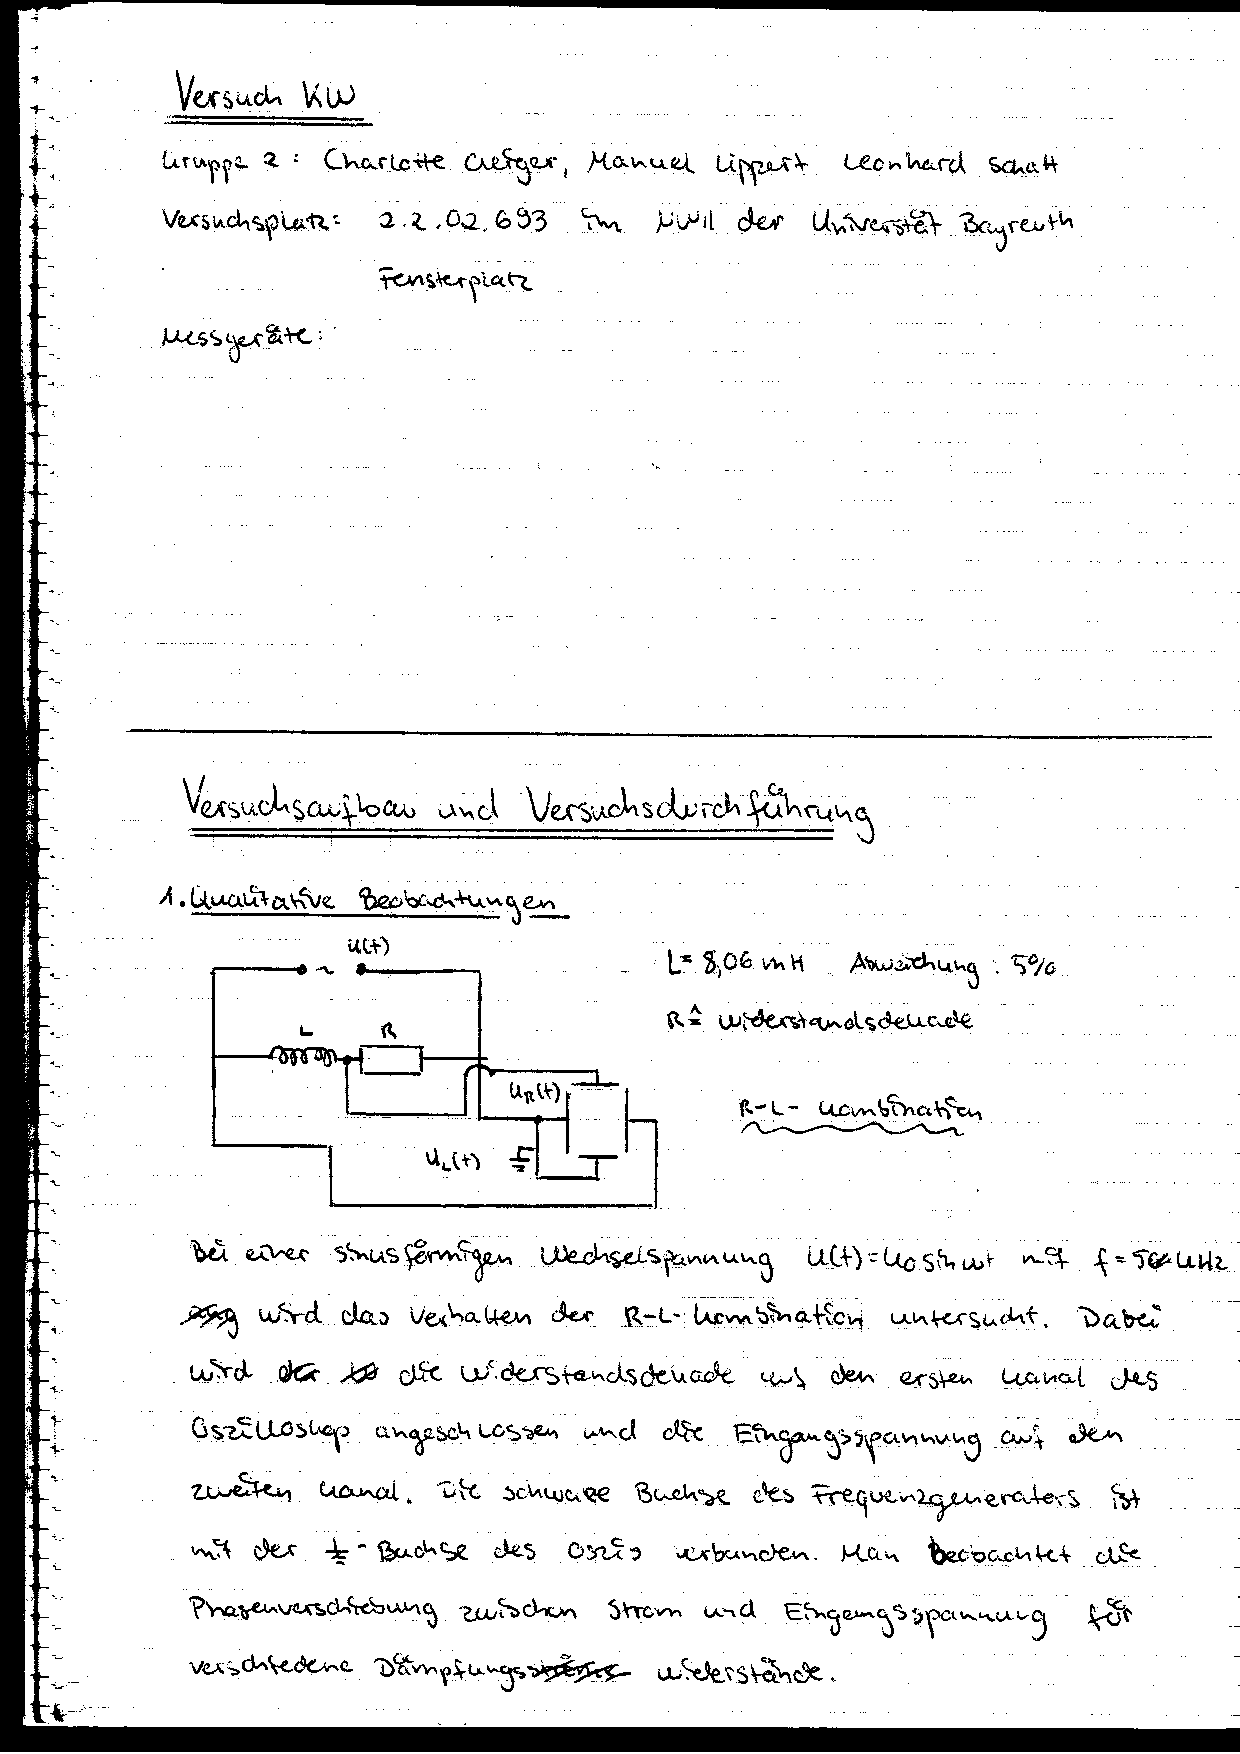
\includegraphics[scale=0.5]{Bilder/Protokoll.PNG}
    \caption{Anregungslaserlinien und Detektionsbereiche zur Lebenszeitmessung an CFP/YFP. }
    \label{fig:laserlinien}
   \end{figure}

